\fancychapter{Clustering Tweets with Self-Organizing Maps}
\label{ch:clustering_tweets}

Tweets categorization with \ac{SOMs} requires a dataset to work on. Due to systematic API restrictions, which where implemented in order to protect Twitter business model, gathering a dataset that directly maps to the social network is a great challenge by itself. 
In order to categorize tweets with \ac{SOMs} first we used a dataset provided by INESC-ID. The dataset had almost 1TB of data in \ac{JSON} format.

\section{Dataset Characteristics}
\label{sec:dataset_characteristics}

Each tweet is comprised of multiple parameters. Figure~\ref{fig:json_tweet} shows how a tweet is represented in \ac{JSON} format. Inside the tweet there is also information about the user whom created the tweet, shown in Figure~\ref{fig:json_tweet_user} and entities shown in Figure~\ref{fig:tweet_enteties}.

As can be seen in Figure~\ref{fig:json_tweet_user} no information about the social relations of the user which emitted the tweet are present. Therefor in order to retrieve the social network in which a user is contained, it will be necessary to connect to the Twitter API. Crawling twitter is discussed in further depth in Chapter~\ref{chap:crawling_twitter}.  

\begin{figure}
  \begin{center}
    \begin{lstlisting}[language=json,firstnumber=1]
{ 
  "_id" : { "$oid" : "4fa14bc97e5617025fb14787" },
  "text" : "RT @FastCoDesign: A Paintbrush That Works On The iPad http://t.co/eWjEZAga (@sensubrushman)",
  "id_str" : "197701817864421376", 
  "coordinates" : null, 
  "in_reply_to_screen_name" : null, 
  "in_reply_to_user_id" : null,
  "possibly_sensitive" : false, 
  "favorited" : false, 
  "in_reply_to_status_id" : null, 
  "source" : "<a href=\"http://www.flipboard.com\" rel=\"nofollow\">Flipboard</a>", 
  "possibly_sensitive_editable" : true, 
  "contributors" : null, 
  "retweet_count" : 0, 
  "truncated" : false,
  "in_reply_to_status_id_str" : null,
  "geo" : null,
  "in_reply_to_user_id_str" : null,
  "entities" : { Enteties Object },
  "user" : { User object },
  "retweeted" : false,
  "id" : 197701817864421376,
  "place" : null,
  "created_at" : "Wed May 02 14:59:21 +0000 2012" }

    \end{lstlisting}
  \end{center}
  \caption{\ac{JSON} representation of a Tweet.}
  \label{fig:json_tweet}
\end{figure}



% \begin{figure}
  \centering
    \begin{lstlisting}[language=json,firstnumber=1]
 { "user_mentions" : 
   [{ "indices" : [ 3, 16 ], 
     "id_str" : "158865339",
     "name" : "Co.Design",
     "id" : 158865339,
     "screen_name" : "FastCoDesign" },
   { "indices" : [ 76, 90 ], 
     "id_str" : "534544812",
     "name" : "Matt",
     "id" : 534544812,
     "screen_name" : "sensubrushman" } ],
   "urls" :
     [ { "url" : "http://t.co/eWjEZAga",
         "indices" : [ 54, 74 ], "display_url" : "bit.ly/IAaKQf",
         "expanded_url" : "http://bit.ly/IAaKQf" } ],
   "hashtags" : [] }
    \end{lstlisting}
  \caption{Enteties mentioned inside the tweet}
  \label{fig:tweet_enteties}
\end{figure}

%\begin{figure}
  \begin{center}
    \begin{lstlisting}[language=json,firstnumber=1]
    { "default_profile_image" : false,
      "friends_count" : 277,
      "profile_link_color" : "0084B4",
      "followers_count" : 105,
      "url" : null,
      "profile_image_url" : "http://a0.twimg.com/profile_images/690647919/19335_266330051104_635886104_3750428_5949465_n_normal.jpg",
      "id_str" : "26549290",
      "following" : null,
      "favourites_count" : 7,
      "notifications" : null,
      "profile_background_color" : "C0DEED",
      "statuses_count" : 331,
      "profile_background_tile" : false,
      "profile_background_image_url_https" : "https://si0.twimg.com/profile_background_images/79871480/DSC09031_2.jpg",
      "description" : "A Chicago-based designer and educator fascinated with the power of design to ignite change \r\n\r\n",
      "location" : "Chicago",
      "contributors_enabled" : false,
      "geo_enabled" : false,
      "time_zone" : "Central Time (US & Canada)",
      "profile_sidebar_fill_color" : "cde2e6",
      "listed_count" : 2,
      "profile_sidebar_border_color" : "C0DEED",
      "default_profile" : false,
      "show_all_inline_media" : false,
      "verified" : false,
      "protected" : false,
      "is_translator" : false,
      "profile_use_background_image" : true,
      "profile_image_url_https" : "https://si0.twimg.com/profile_images/690647919/19335_266330051104_635886104_3750428_5949465_n_normal.jpg",
      "name" : "Karma Dabaghi",
      "follow_request_sent" : null,
      "lang" : "en",
      "profile_text_color" : "333333",
      "id" : 26549290,
      "profile_background_image_url" : "http://a0.twimg.com/profile_background_images/79871480/DSC09031_2.jpg",
      "utc_offset" : -21600,
      "created_at" : "Wed Mar 25 17:55:26 +0000 2009",
    "screen_name" : "karmadabaghi"  }
    \end{lstlisting}
  \end{center}
  \caption{\ac{JSON} representation of a user, inside a tweet.}
  \label{fig:json_tweet_user}
\end{figure}


In order to better understand the dataset at hand, all the \ac{JSON} files where converted into \ac{CSV}in a way to reduce the size of the dataset. While tweets where being converted, \ac{URL} where removed --- since most of them where minified in order to fit in less that 140 characters, without translating the minified URL, not a lot of information can be gathered. Also, all tweets that where not identified as being in English where also removed. The tweet shown in \ac{JSON} format in Figure~\ref{fig:json_tweet} is converted to \ac{CSV} in Figure~\ref{fig:csv_tweet}.

\begin{figure}
  \begin{center}
    \begin{lstlisting}[language=json,firstnumber=1]
    karmadabaghi,A Paintbrush That Works On The iPad @sensubrushman
    \end{lstlisting}
  \end{center}
  \caption{\ac{CSV} representation of a Tweet. The username is present in the first column and the tweet text on the last.}
  \label{fig:csv_tweet}
\end{figure}


{\color{red} Add table with dataset characteristics }
%\begin{tabular}{c | c}
  %Number of Files  & 337\\
  %Average File Size  & 337\\
%\end{tabulartabular}


\section{Initial SOM training}
\label{sec:ininitial_som_trainning}

{\color{red} Describe naive approach to SOM training in R }
{\color{red} Describe amount of weird words }

\subsection{Reducing SOM vector size}
\label{sub:reducing_som_vector_size}

\subsubsection{Identify Tweets language}
\label{ssub:identify_tweets_lang}

Identifying tweets that where not in the English language was done through the usage of Ruby library called whatlanguage~\footnote{https://github.com/peterc/whatlanguage}, which tries to identify one language through Bloom Filters. Inside the tweet there is a field which identifies the user language, we found that x is not acurate. Removing tweets that weren't in the english language reduced the amount of different words in x and therefor will reduce the dimensional size of the \ac{SOM}.

{\color{red}  The initial dataset features is described table x}
 .
\subsubsection{Text Manipulation for VSM reduction}
\label{ssub:Text Manipulation for SVM reduction}
{\color{red} all the text techniques used }
{\color{red} show amount of words reduction with the introduction of a new technique and the amount of time that it takes to be applied }

Work done on the INESC twitter dataset with SOMs.
SOM implementations used, what where their strong points and weaknesses

\subsubsection{Clustering with Word Selection }
\label{ssub:Word Selection for Clustering}
{\color{red} Results of SOMs using selected words based on occurrence after applying SVM reduction }
{\color{red} Results where pretty bad }

\subsection{Intermediate Conclusions}
\label{sub:intermediate_conclusions}
{\color{red} Only these methods are not enough to cluster tweets }

\subsection{Clustering with NLP selected words}
\label{sub:clustering_with_nlp_selected_words}
{\color{red} results of som using arktweet NLP }
{\color{red} types of tags selected }
{\color{red} show tweets that had no representation }
{\color{red} review clusters and results }


\section{Conclusions}
\label{sec:conclusions}


\fancychapter{Crawling Twitter for Social Relations}
\label{chap:crawling_twitter}
The INESC twitter dataset, was a good dataset to start analyzing the complexity of clustering tweets. On Chapter \ref{ch:clustering_tweets} we deeply analyzed the characteristics of the INESC twitter dataset, and concluded that it was not optimal to the problem we are trying to solve since it doesn't have the social connections between the authors of the tweets. This problem could be solved in any of the following ways:
\begin{itemize}
  \item \textbf{First aproach: } For each tweet, fetch the user information including the users he is connected to.
  \item \textbf{Second aproach: } Create our own crawler, where the social connections, tweets and users are saved.
\end{itemize}

As described in {\color{red} add reference to the amount of users that no longer exists that will be somewhere on a table where the daset is resumed } there is an x\% of users that are not accessible or have terminated their account. This complicates the process of crawling due to twitter API limits, since every time we try to download information from a non existing user we: a) don't receive any data, and b) just burned an API request --- we could ask for maximum of 100 users per request, we can only make 15 requests per 15 minute window --- . Another problem is that, as soon as we got the available users and actually issued new requests to get a user list of followers, we are limited to only 15 requests per 15 minute window. Finally the average date of publication of the tweets is about {\color{red} verify average date }, getting the actual followers of a user might not even reflect the tweet he made a couple of years a go --- specially with all the Justin Beaber obsession present in the dataset {\color{red} ref more common words }.

Due to all these reasons we decided to create our own crawler and download our own slice of twitter.

\section{Twitter Crawler}
\label{sec:twitter_crawler}
When designing the twitter crawler, we took into consideration that it had to be extremely resilient in order to be able to be left alone, crawling the twitter, until told to stop. Also if anything happened to the machine where the crawler was running it would be necessary to return to some previous crawling state, with minimum data loss. Algorithm {\color{red} I NEED TO WRITE THIS ALGORITHM } shows the crawler algorithm, which works in the following way:

\begin{itemize}
  \item \textbf{Step 1:} Choose some seed users to start crawling or deserialize a serialized version of the crawler if available.
  \item \textbf{Step 2:} For each seed user get all of his followers, and add them to an array if they haven't yet been crawled.
  \item \textbf{Step 3:} Repeat step one with random users taken from the array on step 2, until API limit is reached.
  \item \textbf{Step 4:} When API limit is reached, print the state of the crawled network, serialize the current state, and wait 15 minutes until it is possible to resume crawling. 
\end{itemize}

\subsection{Crawler Performance}
\label{sub:crawler_performance}
{\color{red} show number of tweets per second, number user per second, and users reached per second. }
{\color{red} compare the with the theoretical maximum }
{\color{red} compare size of the serialized social network with the amount of tweets and users it is getting  }
{\color{red} compare time taken to deserialize with amount of tweets crawled }
{\color{red} compare time to serialize with amount of tweets crawled }

%Explain the limitations of the INESC tweet dataset: crawlled by hashtag, social connections can only be obtained through connections to the twitter API, a lot of the tweets had no active users etc. 

\fancychapter{SOM Framework}
{\color{red} Resume this chapter }

\section{Motivation}
\label{sec:motivation}
When researching ways to extend the \ac{SOM} algorithm, in order to add social features to the learning process. I found that the number of \ac{SOM} libraries was not very extense. Even though, programing languages often used in \ac{ML} and Data Mining, such as Python or C++, have their how implementation of the \ac{SOM} algorithm. I've found that most of these libraries are made in such a way to be extremely fast, in order to take as much advantage from the hardware they are running on as possible. They often lack the modularity needed to adapt the \ac{SOM} algorithm to specific problems.

The \ac{SOM} algorithm has been changed many times in order to better categorize data with specific features, for example Geo-SOM was described in Subsection~\ref{sub:types_of_soms}, the Growing Hierarchical SOM~\cite[]{1058070}, the time adaptive SOM~\cite[]{1187438}, the Ontological SOM~\cite[]{5446427}, and the list goes on\dots  

In order to create the homophilic SOM, described in Section~\ref{sec:algorithm_changes} we first created a SOM framework that is easy to extend due to be fully object oriented, scripted --- even though it can be compiled to run on the JVM --- and without C extensions.

\section{Implementation}
\label{sec:implementation}
The \ac{SOM} framework was developed in the Ruby programing language \footnote{https://www.ruby-lang.org/en/} due to the desired characteristic of allowing great levels of introspection and being an almost pure object oriented programing language. Due to this characteristics making modifications to core parts of the algorithm is fairly easy.

{\color{red} Descrevo a organizacao do codigo classes, etc? }

The \ac{SOM} Framework was developed in a test driven fashion, having 100\% of its public methods tested and documented for expected behavior. These characteristics, associated with the fact that was published under an open source license, makes it available for other researchers to implement their own SOM variants.

By default, the base SOM algorithm is implemented as described by the Algorithm~\ref{alg:som} in Section \ref{sec:the_self_organizing_map}. 
\subsection{Clustering Color Vectors}
\label{sub:main_features}
Out of the box, the \ac{SOM} Framework implements a squared output space, where all residing neurons are manipulated as arrays. It is possible ate any given moment of the training to export the output space to \ac{JSON}, \ac{CSV} or to visualize its current \ac{U-Matrix}. Also during training a progress bar is displayed in order to know how much time will be needed for the training to end.

Due to the features described above, it is possible to train a \ac{SOM} to identify random colors --- RGB vectors --- while printing the results. In order to do this we will start by:
\begin{itemize}
  \item Initializing a SOM object with an output space size of 15 by 15 neurons, which will yield a total of 255 neurons --- and directly maps to the maximum number of clusters --- and 700 epochs.
  \item Create 1500 input patterns with size 3 and random values between 0 and 255. 
  \item Tell the SOM to print its state at the end of each epoch.
\end{itemize}
The machine used for training had the hardware specifications outlined in table \ref{tab:mac_test}

\begin{table}[H]
  \caption{Test machine one specs}
  \label{tab:mac_test}
  \begin{center}
    \begin{tabular}{|c|c|}
      \hline
      Operative System & OSX 10.9.5 \\
      \hline
      Memory           & 8 GB, 1067MHz DDR3       \\
      \hline
      Processor        & 2,4GHz Intel Core 2  Duo \\
      \hline
      Hard Drive       & 128GB SSD  \\
      \hline
    \end{tabular}
  \end{center}
\end{table}


A summary of the training is specified in Table~\ref{tab:som_colours}
\begin{table}[H]
  \caption{SOM trainning resumed}
  \label{tab:som_colours}
  \begin{center}
    \begin{tabular}{|c|c|}
      \hline
      \textbf{Number of Neurons} & 225 \\
      \hline
      \textbf{Output Space Size} & 15x15 \\
      \hline
      \textbf{Number of Input Patterns} & 1500 \\
      \hline
      \textbf{VSM size of Input Patterns and Neurons} & 3 \\
      \hline
      \textbf{Number of Epochs} & 600 \\
      \hline
      \textbf{Training Duration} & 14 hours \\
      \hline
      \textbf{Type of Train} & print each epoch training\\
      \hline
      \textbf{Initial learning rate} & 0.6\\
      \hline
      \textbf{Initial Radius} & 8\\
      \hline
    \end{tabular}
  \end{center}
\end{table}


\begin{figure}[h]
  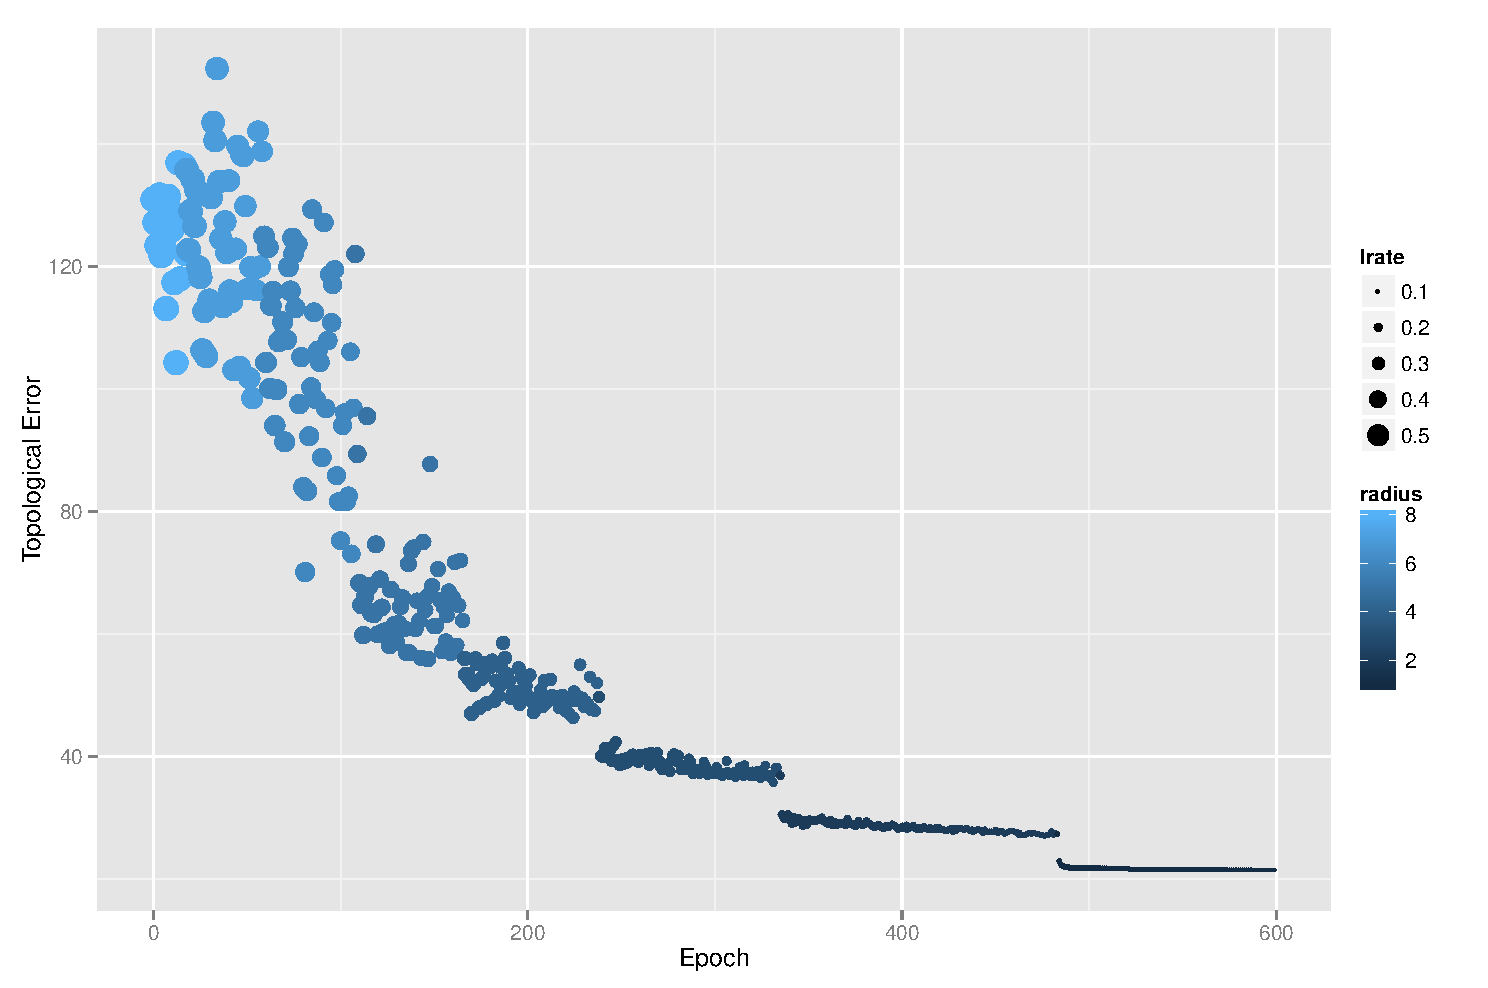
\includegraphics[scale=0.6]{./plots/som/topological_error.pdf}
  \label{fig:top_error}
  \caption{Changes in topological error throughout the SOM training, lrate stands for learning rate, and radius for radius applied to the winning neuron}
\end{figure}

\begin{figure}[h]
  \centerline{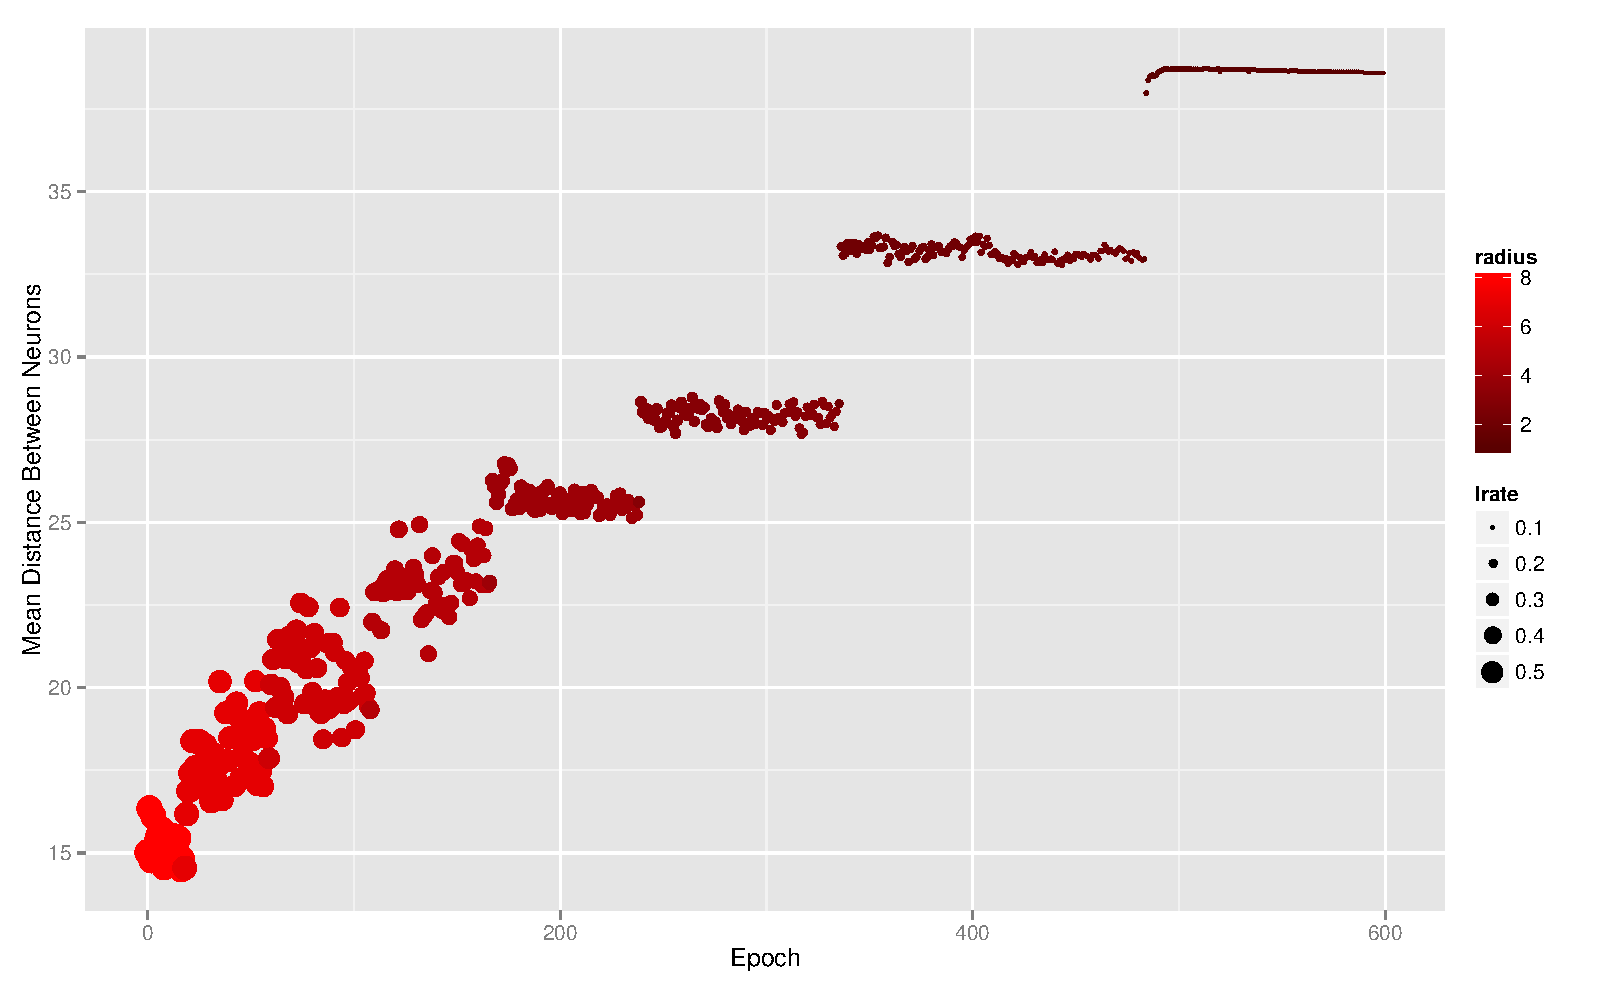
\includegraphics[scale=0.6]{./plots/som/average_distance.pdf}}
  \label{fig:avg_dist}
  \caption{Changes in the average distance between neurons, throughout the SOM training}
\end{figure}

\begin{figure}[htpb]
  \centering
  \subfigure[Output Space]{
\includegraphics[scale=1]{./images/som_training/1_som.pdf}\label{chp3:onesom}}
  \hspace*{0.5cm}
  \subfigure[U-Matrix]{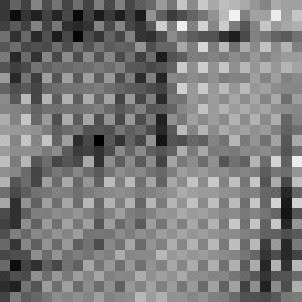
\includegraphics[scale=0.5]{./images/som_training/1_umatrix.pdf}\label{chp3:onematrix}}
  \hspace*{0.5cm}
  \subfigure[Q-Matrix]{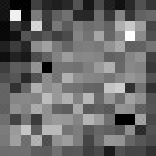
\includegraphics[scale=1]{./images/som_training/1_quantmatrix.pdf}\label{chp3:onetopmat}}
  \hspace*{0.5cm}
  \caption{ SOM state after first epoch of training. Its learning rate is at 0.598, and radius at 8.  }
  \label{fig:}
\end{figure}

\begin{figure}[htpb]
  \centering
  \subfigure[Output Space]{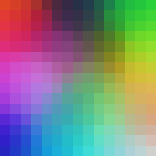
\includegraphics[scale=1]{./images/som_training/2_som.pdf}\label{chp3:onesom}}
  \hspace*{0.5cm}
  \subfigure[U-Matrix]{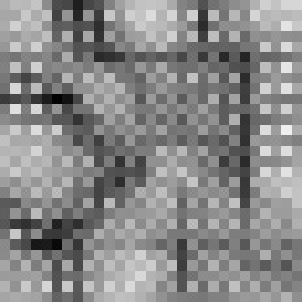
\includegraphics[scale=0.5]{./images/som_training/2_umatrix.pdf}\label{chp3:onematrix}}
  \hspace*{0.5cm}
  \subfigure[Q-Matrix]{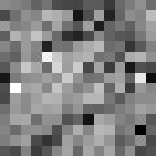
\includegraphics[scale=1]{./images/som_training/2_quantmatrix.pdf}\label{chp3:onetopmat}}
  \hspace*{0.5cm}
  \caption{ SOM state after second epoch of training. Its learning rate is at 0.22, and radius at 3.  }
  \label{fig:}
\end{figure}

\begin{figure}[htpb]
  \centering
  \subfigure[Output Space]{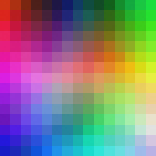
\includegraphics[scale=1]{./images/som_training/3_som.pdf}\label{chp3:onesom}}
  \hspace*{0.5cm}
  \subfigure[U-Matrix]{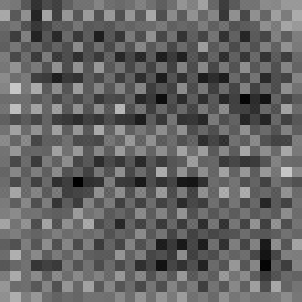
\includegraphics[scale=0.5]{./images/som_training/3_umatrix.pdf}\label{chp3:onematrix}}
  \hspace*{0.5cm}
  \subfigure[Q-Matrix]{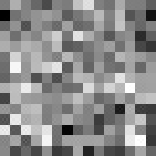
\includegraphics[scale=1]{./images/som_training/3_quantmatrix.pdf}\label{chp3:onetopmat}}
  \hspace*{0.5cm}
  \caption{ SOM state after third epoch of training. Its learning rate is at 0.081, and radius at 1.  }
  \label{fig:}
\end{figure}

\begin{figure}[htpb]
  \centering
  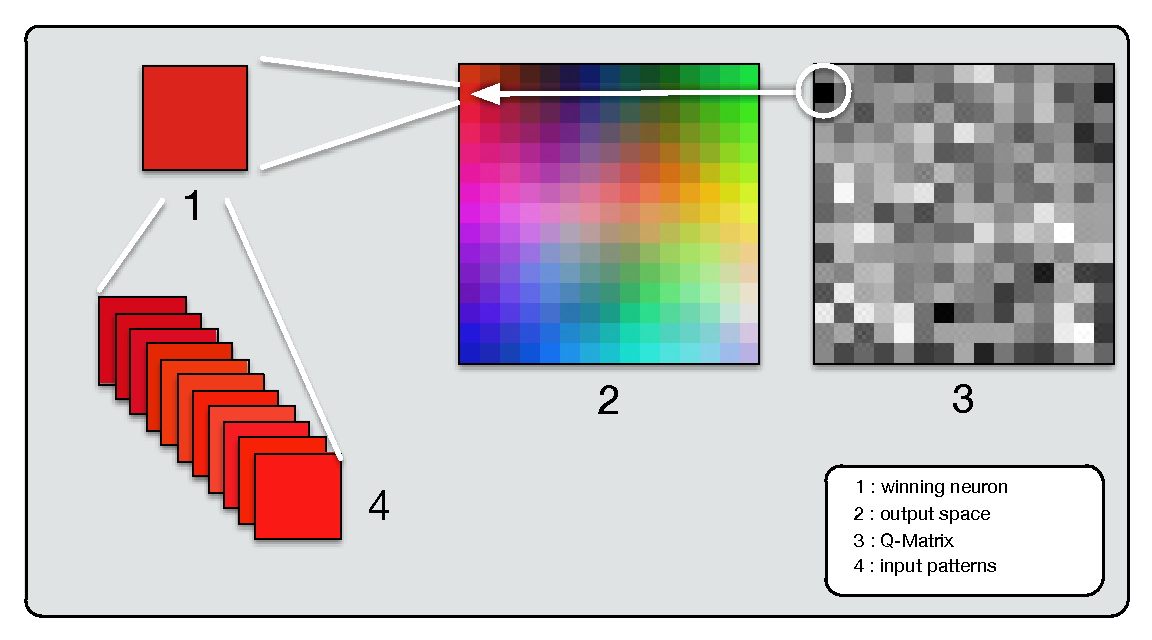
\includegraphics[width=0.8\linewidth]{./images/som_trainned.pdf}
  \caption{Input patterns associated with the neuron with maximum topological error --31. Even though the neuron has the biggest topological error of all neurons, it still has a good representation of the input patterns. The colors in this image are not figurative, and represent the entities at the end of trainning  }
  \label{fig:./images/som_trainned}
\end{figure}

\subsection{Benchmarking}
\label{sub:benchmarking}


%Explain what got me to create my own ruby library: everybody is making their own SOM algorithms ( ex.: websom, hsom etc ). Most implementations want to get as close to the metal as possible in order to deliver faster trainings, which makes the lybraries hard to modify. SOM framework is an modular implementation of the SOM algorithm in an higher level programing language which makes it easier to construct and test new SOM algorithms.

\fancychapter{Clustering Socially Connected Data}
The default \ac{SOM} algorithm has no idea whatsoever of the social connections between the tweets, it simply looks at the binary vectors that represent sentences and assigns it to the most similar neuron.

In order to better categorize socially connected data, we propose some alterations to the \ac{SOM} algorithm in order to make it aware of the social connections between the tweets, and therefor better represent the homophilic behavior present on social networks.

{\color{red} insert homophilic som algorith here}

\section{Homophilic SOM Definition}
\label{sec:algorithm_changes}

\subsection{Output Space}
\label{sub:output_space}
The outputs space is the zone on the \ac{SOM} algorithm where the neurons reside. It works like a cortex where neurons are scattered in a geometric fashion, generally a square. The output space is generally initialized with random values, with a relatively high learning rate, and also a relatively high number of epochs. The algorithm is made this way in order to be able to identify any type of data that can be represented as vectors.

First we will try to change the output space to better resemblance the social network. In order to do this, the squared grid that defines the output space was changed by the social network connections, and the neurons, are represented by a social network user. This changes are applied in the following way:
\begin{figure}[htpb]
  \centering
  \subfigure[The neighbourhood is defined by the relations of followers/followees between the winning neuron and the other neurons]{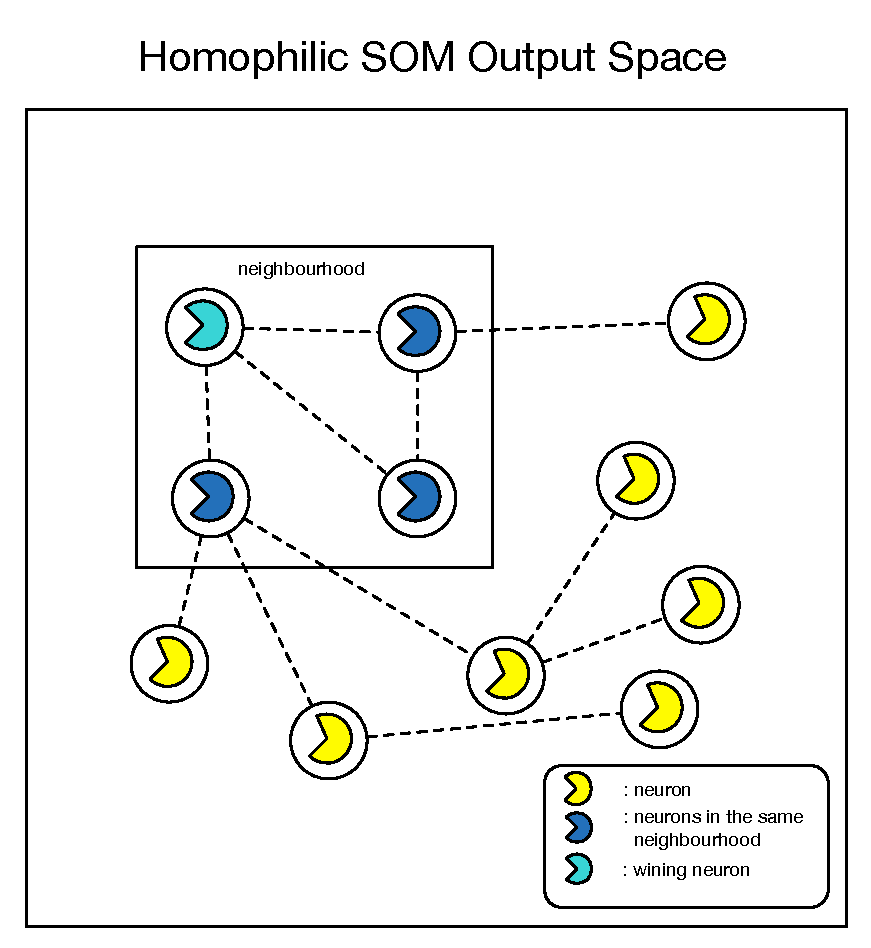
\includegraphics[scale=0.3]{./images/homophilic_outputspace.pdf}\label{chp3:homout}}
  \hspace*{0.5cm}
  \subfigure[Homophilic input space works in the same way as a normal input space]{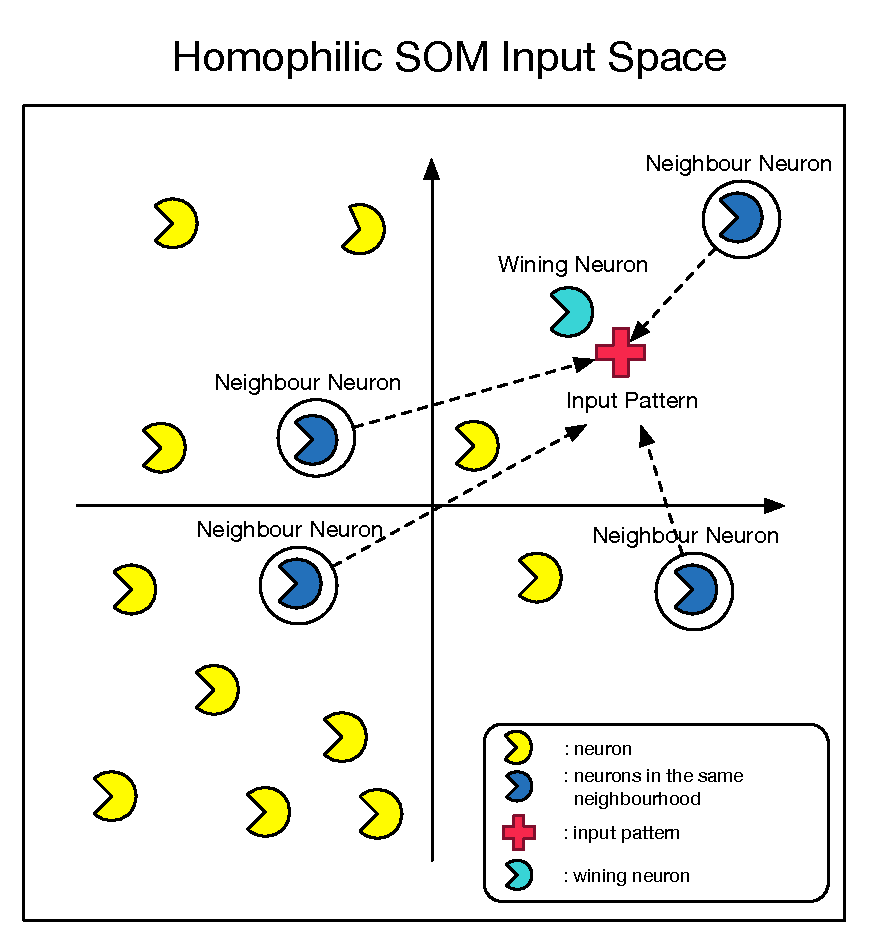
\includegraphics[scale=0.3]{./images/homophilic_input_space.pdf}\label{chp3:homin}}
  \label{fig:homo_in_out}
  \caption{ Homophilic SOM output and input space during the learning phase. }
\end{figure}
\begin{itemize}
  \item Each neuron is comprised of the text from all the tweets that he authored.
  \item Each neuron has a unique id, and stores the ids of his followers and followees that are present in the output space.
  \item During the learning phase, the radius will be defined as the maximum number of hops separating the winning neuron and followers/followees of followers/followees. 
  %\item Each neuron will cache followers/followees of a follower/followee to a specified depth level, for performance purposes. 
\end{itemize}

{\color{red} insert image of the output space with social features vrs tipical output space}

\subsection{Learning Phase}
\label{sub:learning_phase}
Like in the default \ac{SOM} the learning phase is where the output space is trained in order to organize the input data into clusters. Since this algorithm is specific to categorize tweets using social network features, the learning rate, radius and number of epochs used can be greatly reduced in order for the algorithm to converge. The learning phase operates in the following way:

\begin{itemize}
  \item The distance between the input pattern and all the neurons is calculated. The neuron closest to the input pattern is considered the winning neuron.
  \item When the winning neuron is selected, he and his social neighbors within k hops, update their representations in the input space, and move closer to the input patter. The Gaussian function (Func.~\ref{eq:gaussian}) is also used in here in order for the neighbors that are closer to the input pattern be significantly more influenced by the input pattern, while the neurons further away are less influenced. 
  \item This process is repeated for a predefined number of epochs. While the number of epochs increases, the learning rate, and number of hops that defines the neighborhood decreases in order for the algorithm to converge.
\end{itemize}

Just like the default \ac{SOM} algorithm, after the map is trained, input patterns can be fast assign to the nearest neuron since the neuron positions in the output space are no longer updated.

{\color{red} Link to the learning phase in the algorithm on the main chapter, add images of the training model }

\section{Social Clusters}
\label{sec:hmophilic_som_clusters}
{\color{red} resume what is written in this chapter }

\subsection{Training}
\label{sub:dataset}
In order to train the Homophilic SOM, we used the crawler defined in Section~\ref{sec:data_mining_in_twitter_}. The dataset had the following characteristics:
{\color{red} add table with number of users, tweets, tags, on the dataset}
{\color{red} show amount of time it took to train the SOM}
{\color{red} show umatrixes of the trainne }
{\color{red} compare clusters/time and umatrixes of the default SOM and the Homophilic SOM}
{\color{red} show the tweets in some clusters }


